\documentclass[twoside]{book}

% Packages required by doxygen
\usepackage{fixltx2e}
\usepackage{calc}
\usepackage{doxygen}
\usepackage[export]{adjustbox} % also loads graphicx
\usepackage{graphicx}
\usepackage[utf8]{inputenc}
\usepackage{makeidx}
\usepackage{multicol}
\usepackage{multirow}
\PassOptionsToPackage{warn}{textcomp}
\usepackage{textcomp}
\usepackage[nointegrals]{wasysym}
\usepackage[table]{xcolor}

% Font selection
\usepackage[T1]{fontenc}
\usepackage[scaled=.90]{helvet}
\usepackage{courier}
\usepackage{amssymb}
\usepackage{sectsty}
\renewcommand{\familydefault}{\sfdefault}
\allsectionsfont{%
  \fontseries{bc}\selectfont%
  \color{darkgray}%
}
\renewcommand{\DoxyLabelFont}{%
  \fontseries{bc}\selectfont%
  \color{darkgray}%
}
\newcommand{\+}{\discretionary{\mbox{\scriptsize$\hookleftarrow$}}{}{}}

% Page & text layout
\usepackage{geometry}
\geometry{%
  a4paper,%
  top=2.5cm,%
  bottom=2.5cm,%
  left=2.5cm,%
  right=2.5cm%
}
\tolerance=750
\hfuzz=15pt
\hbadness=750
\setlength{\emergencystretch}{15pt}
\setlength{\parindent}{0cm}
\setlength{\parskip}{3ex plus 2ex minus 2ex}
\makeatletter
\renewcommand{\paragraph}{%
  \@startsection{paragraph}{4}{0ex}{-1.0ex}{1.0ex}{%
    \normalfont\normalsize\bfseries\SS@parafont%
  }%
}
\renewcommand{\subparagraph}{%
  \@startsection{subparagraph}{5}{0ex}{-1.0ex}{1.0ex}{%
    \normalfont\normalsize\bfseries\SS@subparafont%
  }%
}
\makeatother

% Headers & footers
\usepackage{fancyhdr}
\pagestyle{fancyplain}
\fancyhead[LE]{\fancyplain{}{\bfseries\thepage}}
\fancyhead[CE]{\fancyplain{}{}}
\fancyhead[RE]{\fancyplain{}{\bfseries\leftmark}}
\fancyhead[LO]{\fancyplain{}{\bfseries\rightmark}}
\fancyhead[CO]{\fancyplain{}{}}
\fancyhead[RO]{\fancyplain{}{\bfseries\thepage}}
\fancyfoot[LE]{\fancyplain{}{}}
\fancyfoot[CE]{\fancyplain{}{}}
\fancyfoot[RE]{\fancyplain{}{\bfseries\scriptsize Generated by Doxygen }}
\fancyfoot[LO]{\fancyplain{}{\bfseries\scriptsize Generated by Doxygen }}
\fancyfoot[CO]{\fancyplain{}{}}
\fancyfoot[RO]{\fancyplain{}{}}
\renewcommand{\footrulewidth}{0.4pt}
\renewcommand{\chaptermark}[1]{%
  \markboth{#1}{}%
}
\renewcommand{\sectionmark}[1]{%
  \markright{\thesection\ #1}%
}

% Indices & bibliography
\usepackage{natbib}
\usepackage[titles]{tocloft}
\setcounter{tocdepth}{3}
\setcounter{secnumdepth}{5}
\makeindex

% Hyperlinks (required, but should be loaded last)
\usepackage{ifpdf}
\ifpdf
  \usepackage[pdftex,pagebackref=true]{hyperref}
\else
  \usepackage[ps2pdf,pagebackref=true]{hyperref}
\fi
\hypersetup{%
  colorlinks=true,%
  linkcolor=blue,%
  citecolor=blue,%
  unicode%
}

% Custom commands
\newcommand{\clearemptydoublepage}{%
  \newpage{\pagestyle{empty}\cleardoublepage}%
}

\usepackage{caption}
\captionsetup{labelsep=space,justification=centering,font={bf},singlelinecheck=off,skip=4pt,position=top}

%===== C O N T E N T S =====

\begin{document}

% Titlepage & ToC
\hypersetup{pageanchor=false,
             bookmarksnumbered=true,
             pdfencoding=unicode
            }
\pagenumbering{alph}
\begin{titlepage}
\vspace*{7cm}
\begin{center}%
{\Large embedded\+\_\+project\+\_\+template }\\
\vspace*{1cm}
{\large Generated by Doxygen 1.8.13}\\
\end{center}
\end{titlepage}
\clearemptydoublepage
\pagenumbering{roman}
\tableofcontents
\clearemptydoublepage
\pagenumbering{arabic}
\hypersetup{pageanchor=true}

%--- Begin generated contents ---
\chapter{File Index}
\section{File List}
Here is a list of all documented files with brief descriptions\+:\begin{DoxyCompactList}
\item\contentsline{section}{/home/andressanchez/\+Escritorio/\+G\+I\+T/project\+\_\+template/src/drivers/\hyperlink{drv__hrt_8h}{drv\+\_\+hrt.\+h} }{\pageref{drv__hrt_8h}}{}
\item\contentsline{section}{/home/andressanchez/\+Escritorio/\+G\+I\+T/project\+\_\+template/src/drivers/\hyperlink{drv__orb__dev_8h}{drv\+\_\+orb\+\_\+dev.\+h} }{\pageref{drv__orb__dev_8h}}{}
\item\contentsline{section}{/home/andressanchez/\+Escritorio/\+G\+I\+T/project\+\_\+template/src/include/\hyperlink{visibility_8h}{visibility.\+h} }{\pageref{visibility_8h}}{}
\item\contentsline{section}{/home/andressanchez/\+Escritorio/\+G\+I\+T/project\+\_\+template/src/include/containers/\hyperlink{IntrusiveSortedList_8hpp}{Intrusive\+Sorted\+List.\+hpp} }{\pageref{IntrusiveSortedList_8hpp}}{}
\item\contentsline{section}{/home/andressanchez/\+Escritorio/\+G\+I\+T/project\+\_\+template/src/include/containers/\hyperlink{List_8hpp}{List.\+hpp} }{\pageref{List_8hpp}}{}
\item\contentsline{section}{/home/andressanchez/\+Escritorio/\+G\+I\+T/project\+\_\+template/src/include/containers/{\bfseries Lock\+Guard.\+hpp} }{\pageref{LockGuard_8hpp}}{}
\item\contentsline{section}{/home/andressanchez/\+Escritorio/\+G\+I\+T/project\+\_\+template/src/lib/cdev/\hyperlink{CDev_8cpp}{C\+Dev.\+cpp} }{\pageref{CDev_8cpp}}{}
\item\contentsline{section}{/home/andressanchez/\+Escritorio/\+G\+I\+T/project\+\_\+template/src/lib/cdev/\hyperlink{CDev_8hpp}{C\+Dev.\+hpp} }{\pageref{CDev_8hpp}}{}
\item\contentsline{section}{/home/andressanchez/\+Escritorio/\+G\+I\+T/project\+\_\+template/src/lib/cdev/nuttx/\hyperlink{cdev__platform_8cpp}{cdev\+\_\+platform.\+cpp} }{\pageref{cdev__platform_8cpp}}{}
\item\contentsline{section}{/home/andressanchez/\+Escritorio/\+G\+I\+T/project\+\_\+template/src/lib/cdev/nuttx/{\bfseries cdev\+\_\+platform.\+hpp} }{\pageref{cdev__platform_8hpp}}{}
\item\contentsline{section}{/home/andressanchez/\+Escritorio/\+G\+I\+T/project\+\_\+template/src/lib/version/{\bfseries px\+\_\+update\+\_\+git\+\_\+header.\+py} }{\pageref{px__update__git__header_8py}}{}
\item\contentsline{section}{/home/andressanchez/\+Escritorio/\+G\+I\+T/project\+\_\+template/src/lib/version/{\bfseries version.\+c} }{\pageref{version_8c}}{}
\item\contentsline{section}{/home/andressanchez/\+Escritorio/\+G\+I\+T/project\+\_\+template/src/lib/version/\hyperlink{version_8h}{version.\+h} }{\pageref{version_8h}}{}
\item\contentsline{section}{/home/andressanchez/\+Escritorio/\+G\+I\+T/project\+\_\+template/src/modules/hello/{\bfseries hello.\+cpp} }{\pageref{hello_8cpp}}{}
\item\contentsline{section}{/home/andressanchez/\+Escritorio/\+G\+I\+T/project\+\_\+template/src/modules/hello/{\bfseries hello.\+hpp} }{\pageref{hello_8hpp}}{}
\item\contentsline{section}{/home/andressanchez/\+Escritorio/\+G\+I\+T/project\+\_\+template/src/modules/template\+\_\+module/{\bfseries template\+\_\+module.\+cpp} }{\pageref{template__module_8cpp}}{}
\item\contentsline{section}{/home/andressanchez/\+Escritorio/\+G\+I\+T/project\+\_\+template/src/modules/template\+\_\+module/{\bfseries template\+\_\+module.\+h} }{\pageref{template__module_8h}}{}
\item\contentsline{section}{/home/andressanchez/\+Escritorio/\+G\+I\+T/project\+\_\+template/src/modules/u\+O\+R\+B/{\bfseries O\+R\+B\+Set.\+hpp} }{\pageref{ORBSet_8hpp}}{}
\item\contentsline{section}{/home/andressanchez/\+Escritorio/\+G\+I\+T/project\+\_\+template/src/modules/u\+O\+R\+B/\hyperlink{Publication_8hpp}{Publication.\+hpp} }{\pageref{Publication_8hpp}}{}
\item\contentsline{section}{/home/andressanchez/\+Escritorio/\+G\+I\+T/project\+\_\+template/src/modules/u\+O\+R\+B/{\bfseries Publication\+Multi.\+hpp} }{\pageref{PublicationMulti_8hpp}}{}
\item\contentsline{section}{/home/andressanchez/\+Escritorio/\+G\+I\+T/project\+\_\+template/src/modules/u\+O\+R\+B/\hyperlink{Subscription_8cpp}{Subscription.\+cpp} }{\pageref{Subscription_8cpp}}{}
\item\contentsline{section}{/home/andressanchez/\+Escritorio/\+G\+I\+T/project\+\_\+template/src/modules/u\+O\+R\+B/\hyperlink{Subscription_8hpp}{Subscription.\+hpp} }{\pageref{Subscription_8hpp}}{}
\item\contentsline{section}{/home/andressanchez/\+Escritorio/\+G\+I\+T/project\+\_\+template/src/modules/u\+O\+R\+B/{\bfseries Subscription\+Blocking.\+hpp} }{\pageref{SubscriptionBlocking_8hpp}}{}
\item\contentsline{section}{/home/andressanchez/\+Escritorio/\+G\+I\+T/project\+\_\+template/src/modules/u\+O\+R\+B/\hyperlink{SubscriptionCallback_8hpp}{Subscription\+Callback.\+hpp} }{\pageref{SubscriptionCallback_8hpp}}{}
\item\contentsline{section}{/home/andressanchez/\+Escritorio/\+G\+I\+T/project\+\_\+template/src/modules/u\+O\+R\+B/\hyperlink{SubscriptionInterval_8hpp}{Subscription\+Interval.\+hpp} }{\pageref{SubscriptionInterval_8hpp}}{}
\item\contentsline{section}{/home/andressanchez/\+Escritorio/\+G\+I\+T/project\+\_\+template/src/modules/u\+O\+R\+B/\hyperlink{SubscriptionMultiArray_8hpp}{Subscription\+Multi\+Array.\+hpp} }{\pageref{SubscriptionMultiArray_8hpp}}{}
\item\contentsline{section}{/home/andressanchez/\+Escritorio/\+G\+I\+T/project\+\_\+template/src/modules/u\+O\+R\+B/\hyperlink{uORB_8cpp}{u\+O\+R\+B.\+cpp} }{\pageref{uORB_8cpp}}{}
\item\contentsline{section}{/home/andressanchez/\+Escritorio/\+G\+I\+T/project\+\_\+template/src/modules/u\+O\+R\+B/\hyperlink{uORB_8h}{u\+O\+R\+B.\+h} }{\pageref{uORB_8h}}{}
\item\contentsline{section}{/home/andressanchez/\+Escritorio/\+G\+I\+T/project\+\_\+template/src/modules/u\+O\+R\+B/{\bfseries u\+O\+R\+B\+Common.\+hpp} }{\pageref{uORBCommon_8hpp}}{}
\item\contentsline{section}{/home/andressanchez/\+Escritorio/\+G\+I\+T/project\+\_\+template/src/modules/u\+O\+R\+B/{\bfseries u\+O\+R\+B\+Communicator.\+hpp} }{\pageref{uORBCommunicator_8hpp}}{}
\item\contentsline{section}{/home/andressanchez/\+Escritorio/\+G\+I\+T/project\+\_\+template/src/modules/u\+O\+R\+B/{\bfseries u\+O\+R\+B\+Device\+Master.\+cpp} }{\pageref{uORBDeviceMaster_8cpp}}{}
\item\contentsline{section}{/home/andressanchez/\+Escritorio/\+G\+I\+T/project\+\_\+template/src/modules/u\+O\+R\+B/{\bfseries u\+O\+R\+B\+Device\+Master.\+hpp} }{\pageref{uORBDeviceMaster_8hpp}}{}
\item\contentsline{section}{/home/andressanchez/\+Escritorio/\+G\+I\+T/project\+\_\+template/src/modules/u\+O\+R\+B/{\bfseries u\+O\+R\+B\+Device\+Node.\+cpp} }{\pageref{uORBDeviceNode_8cpp}}{}
\item\contentsline{section}{/home/andressanchez/\+Escritorio/\+G\+I\+T/project\+\_\+template/src/modules/u\+O\+R\+B/{\bfseries u\+O\+R\+B\+Device\+Node.\+hpp} }{\pageref{uORBDeviceNode_8hpp}}{}
\item\contentsline{section}{/home/andressanchez/\+Escritorio/\+G\+I\+T/project\+\_\+template/src/modules/u\+O\+R\+B/{\bfseries u\+O\+R\+B\+Main.\+cpp} }{\pageref{uORBMain_8cpp}}{}
\item\contentsline{section}{/home/andressanchez/\+Escritorio/\+G\+I\+T/project\+\_\+template/src/modules/u\+O\+R\+B/{\bfseries u\+O\+R\+B\+Manager.\+cpp} }{\pageref{uORBManager_8cpp}}{}
\item\contentsline{section}{/home/andressanchez/\+Escritorio/\+G\+I\+T/project\+\_\+template/src/modules/u\+O\+R\+B/{\bfseries u\+O\+R\+B\+Manager.\+hpp} }{\pageref{uORBManager_8hpp}}{}
\item\contentsline{section}{/home/andressanchez/\+Escritorio/\+G\+I\+T/project\+\_\+template/src/modules/u\+O\+R\+B/{\bfseries u\+O\+R\+B\+Topics.\+cpp} }{\pageref{uORBTopics_8cpp}}{}
\item\contentsline{section}{/home/andressanchez/\+Escritorio/\+G\+I\+T/project\+\_\+template/src/modules/u\+O\+R\+B/{\bfseries u\+O\+R\+B\+Topics.\+h} }{\pageref{uORBTopics_8h}}{}
\item\contentsline{section}{/home/andressanchez/\+Escritorio/\+G\+I\+T/project\+\_\+template/src/modules/u\+O\+R\+B/{\bfseries u\+O\+R\+B\+Utils.\+cpp} }{\pageref{uORBUtils_8cpp}}{}
\item\contentsline{section}{/home/andressanchez/\+Escritorio/\+G\+I\+T/project\+\_\+template/src/modules/u\+O\+R\+B/{\bfseries u\+O\+R\+B\+Utils.\+hpp} }{\pageref{uORBUtils_8hpp}}{}
\item\contentsline{section}{/home/andressanchez/\+Escritorio/\+G\+I\+T/project\+\_\+template/src/modules/u\+O\+R\+B/topics/{\bfseries nico.\+h} }{\pageref{nico_8h}}{}
\item\contentsline{section}{/home/andressanchez/\+Escritorio/\+G\+I\+T/project\+\_\+template/src/modules/u\+O\+R\+B/topics/{\bfseries orb\+\_\+test.\+h} }{\pageref{orb__test_8h}}{}
\item\contentsline{section}{/home/andressanchez/\+Escritorio/\+G\+I\+T/project\+\_\+template/src/modules/u\+O\+R\+B/topics/{\bfseries u\+O\+R\+B\+Topics.\+hpp} }{\pageref{uORBTopics_8hpp}}{}
\end{DoxyCompactList}

\chapter{File Documentation}
\hypertarget{visibility_8h}{}\section{/home/andressanchez/\+Escritorio/\+G\+I\+T/project\+\_\+template/src/include/visibility.h File Reference}
\label{visibility_8h}\index{/home/andressanchez/\+Escritorio/\+G\+I\+T/project\+\_\+template/src/include/visibility.\+h@{/home/andressanchez/\+Escritorio/\+G\+I\+T/project\+\_\+template/src/include/visibility.\+h}}
{\ttfamily \#include $<$stdlib.\+h$>$}\newline
{\ttfamily \#include $<$time.\+h$>$}\newline
{\ttfamily \#include $<$pthread.\+h$>$}\newline
{\ttfamily \#include $<$unistd.\+h$>$}\newline
Include dependency graph for visibility.\+h\+:\nopagebreak
\begin{figure}[H]
\begin{center}
\leavevmode
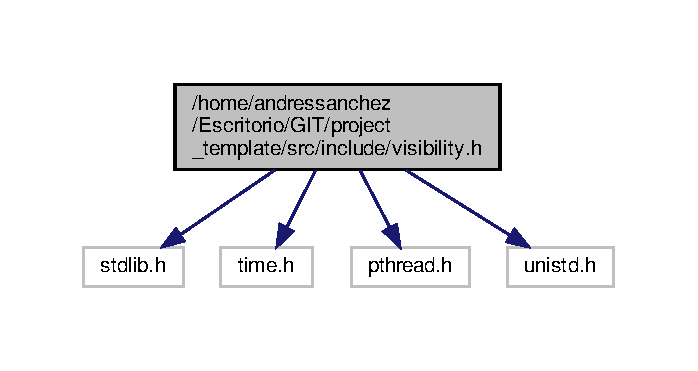
\includegraphics[width=335pt]{de/dda/visibility_8h__incl}
\end{center}
\end{figure}
\subsection*{Macros}
\begin{DoxyCompactItemize}
\item 
\mbox{\Hypertarget{visibility_8h_ad10ef148ba8327bd530fc6c32c1e181c}\label{visibility_8h_ad10ef148ba8327bd530fc6c32c1e181c}} 
\#define {\bfseries \+\_\+\+\_\+\+E\+X\+P\+O\+RT}~\+\_\+\+\_\+attribute\+\_\+\+\_\+ ((visibility (\char`\"{}default\char`\"{})))
\item 
\mbox{\Hypertarget{visibility_8h_aec1804eebbdabd0726d3116f4c48538f}\label{visibility_8h_aec1804eebbdabd0726d3116f4c48538f}} 
\#define {\bfseries \+\_\+\+\_\+\+P\+R\+I\+V\+A\+TE}~\+\_\+\+\_\+attribute\+\_\+\+\_\+ ((visibility (\char`\"{}hidden\char`\"{})))
\item 
\mbox{\Hypertarget{visibility_8h_a568e6bde99652b7fd271ad206cfe38f5}\label{visibility_8h_a568e6bde99652b7fd271ad206cfe38f5}} 
\#define {\bfseries \+\_\+\+\_\+\+B\+E\+G\+I\+N\+\_\+\+D\+E\+C\+LS}
\item 
\mbox{\Hypertarget{visibility_8h_a115472f6d0d1035f1885658ce0821537}\label{visibility_8h_a115472f6d0d1035f1885658ce0821537}} 
\#define {\bfseries \+\_\+\+\_\+\+E\+N\+D\+\_\+\+D\+E\+C\+LS}
\item 
\mbox{\Hypertarget{visibility_8h_a8aff4f29718e32ebdf0ebd54da4cdcc8}\label{visibility_8h_a8aff4f29718e32ebdf0ebd54da4cdcc8}} 
\#define {\bfseries system\+\_\+exit}~exit
\item 
\mbox{\Hypertarget{visibility_8h_a37e5b3149ac079fdc810b883acf34f78}\label{visibility_8h_a37e5b3149ac079fdc810b883acf34f78}} 
\#define {\bfseries system\+\_\+clock\+\_\+gettime}~clock\+\_\+gettime
\item 
\mbox{\Hypertarget{visibility_8h_a6b8f87ca70952144022b8f3871d1e52c}\label{visibility_8h_a6b8f87ca70952144022b8f3871d1e52c}} 
\#define {\bfseries system\+\_\+clock\+\_\+settime}~clock\+\_\+settime
\item 
\mbox{\Hypertarget{visibility_8h_a69c6df7eddd5b4c69515de90386d0ec9}\label{visibility_8h_a69c6df7eddd5b4c69515de90386d0ec9}} 
\#define {\bfseries system\+\_\+pthread\+\_\+cond\+\_\+timedwait}~pthread\+\_\+cond\+\_\+timedwait
\item 
\mbox{\Hypertarget{visibility_8h_ac91f1dfa3a3637967a53e38c9ee6f240}\label{visibility_8h_ac91f1dfa3a3637967a53e38c9ee6f240}} 
\#define {\bfseries system\+\_\+usleep}~usleep
\item 
\mbox{\Hypertarget{visibility_8h_af1e4397aa3029fbee85c47d135f3a4cb}\label{visibility_8h_af1e4397aa3029fbee85c47d135f3a4cb}} 
\#define {\bfseries system\+\_\+sleep}~sleep
\end{DoxyCompactItemize}


\subsection{Detailed Description}
Definitions controlling symbol naming and visibility.

This file is normally included automatically by the build system. 
\hypertarget{version_8h}{}\section{/home/andressanchez/\+Escritorio/\+G\+I\+T/project\+\_\+template/src/lib/version/version.h File Reference}
\label{version_8h}\index{/home/andressanchez/\+Escritorio/\+G\+I\+T/project\+\_\+template/src/lib/version/version.\+h@{/home/andressanchez/\+Escritorio/\+G\+I\+T/project\+\_\+template/src/lib/version/version.\+h}}
{\ttfamily \#include $<$stdint.\+h$>$}\newline
Include dependency graph for version.\+h\+:
\nopagebreak
\begin{figure}[H]
\begin{center}
\leavevmode
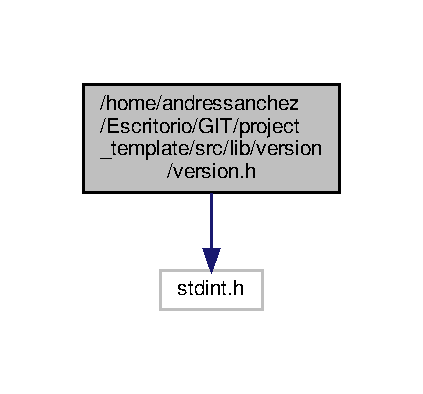
\includegraphics[width=203pt]{d8/d4a/version_8h__incl}
\end{center}
\end{figure}
This graph shows which files directly or indirectly include this file\+:
\nopagebreak
\begin{figure}[H]
\begin{center}
\leavevmode
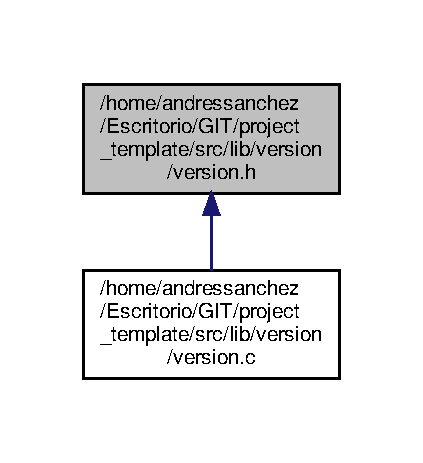
\includegraphics[width=203pt]{d2/deb/version_8h__dep__incl}
\end{center}
\end{figure}
\subsection*{Functions}
\begin{DoxyCompactItemize}
\item 
const char $\ast$ \hyperlink{version_8h_a20fc7c45a2af1951f1bda30a018034cf}{build\+\_\+uri} (void)
\item 
\+\_\+\+\_\+\+E\+X\+P\+O\+RT uint32\+\_\+t \hyperlink{version_8h_ae4d7c8bdf6528ebc410f1aced342f68b}{version\+\_\+tag\+\_\+to\+\_\+number} (const char $\ast$tag)
\item 
\+\_\+\+\_\+\+E\+X\+P\+O\+RT uint32\+\_\+t \hyperlink{version_8h_ade386147dba3b37795fc7f2ec688dd7e}{firmware\+\_\+version} (void)
\item 
\+\_\+\+\_\+\+E\+X\+P\+O\+RT uint32\+\_\+t \hyperlink{version_8h_ab74c0c1be88c621c4649792f2cae5343}{version\+\_\+tag\+\_\+to\+\_\+vendor\+\_\+version\+\_\+number} (const char $\ast$tag)
\item 
\+\_\+\+\_\+\+E\+X\+P\+O\+RT uint32\+\_\+t \hyperlink{version_8h_ae9561a342bd30d0b8e1fdf4393c7e470}{firmware\+\_\+vendor\+\_\+version} (void)
\item 
\+\_\+\+\_\+\+E\+X\+P\+O\+RT uint32\+\_\+t \hyperlink{version_8h_a722e4ea5c20929058c3629578feadaf1}{board\+\_\+version} (void)
\item 
\+\_\+\+\_\+\+E\+X\+P\+O\+RT uint32\+\_\+t \hyperlink{version_8h_a3602739b8e0d5879300a905785c8f371}{os\+\_\+version} (void)
\item 
\+\_\+\+\_\+\+E\+X\+P\+O\+RT const char $\ast$ \hyperlink{version_8h_a5839c1b79b14c6d5c08b1ff84500a971}{os\+\_\+version\+\_\+string} (void)
\item 
\+\_\+\+\_\+\+E\+X\+P\+O\+RT const char $\ast$ \hyperlink{version_8h_a575f337f7a850787f0271320d7859084}{os\+\_\+name} (void)
\item 
\+\_\+\+\_\+\+E\+X\+P\+O\+RT const char $\ast$ \hyperlink{version_8h_a10feca2b0b3de1a3a697cc7bcb90321e}{toolchain\+\_\+name} (void)
\item 
\+\_\+\+\_\+\+E\+X\+P\+O\+RT const char $\ast$ \hyperlink{version_8h_a6df22ceb4e1510ada6b5d742d411b9f9}{toolchain\+\_\+version} (void)
\item 
\+\_\+\+\_\+\+E\+X\+P\+O\+RT const char $\ast$ \hyperlink{version_8h_adb684265d41de587b8ce7eca29392be4}{firmware\+\_\+version\+\_\+string} (void)
\item 
\+\_\+\+\_\+\+E\+X\+P\+O\+RT const char $\ast$ \hyperlink{version_8h_a2705ca759e88988458f05d7d77fc4d87}{firmware\+\_\+git\+\_\+branch} (void)
\item 
\+\_\+\+\_\+\+E\+X\+P\+O\+RT uint64\+\_\+t \hyperlink{version_8h_a1600fb2282c2940e2dffa65585589702}{firmware\+\_\+version\+\_\+binary} (void)
\item 
\+\_\+\+\_\+\+E\+X\+P\+O\+RT const char $\ast$ \hyperlink{version_8h_a740c8b88768645ab5d0754210ebe678c}{ecl\+\_\+lib\+\_\+version\+\_\+string} (void)
\item 
\+\_\+\+\_\+\+E\+X\+P\+O\+RT uint64\+\_\+t \hyperlink{version_8h_a56604d1940f59bed9a41ac57b8f92629}{mavlink\+\_\+lib\+\_\+version\+\_\+binary} (void)
\item 
\+\_\+\+\_\+\+E\+X\+P\+O\+RT uint64\+\_\+t \hyperlink{version_8h_a8534281b0ffc293781e6cd4c04e30e82}{os\+\_\+version\+\_\+binary} (void)
\end{DoxyCompactItemize}


\subsection{Detailed Description}
Tools for system version detection.

\begin{DoxyAuthor}{Author}
Anton Babushkin \href{mailto:anton.babushkin@me.com}{\tt anton.\+babushkin@me.\+com} 

Beat Küng \href{mailto:beat-kueng@gmx.net}{\tt beat-\/kueng@gmx.\+net} 
\end{DoxyAuthor}


\subsection{Function Documentation}
\mbox{\Hypertarget{version_8h_a722e4ea5c20929058c3629578feadaf1}\label{version_8h_a722e4ea5c20929058c3629578feadaf1}} 
\index{version.\+h@{version.\+h}!board\+\_\+version@{board\+\_\+version}}
\index{board\+\_\+version@{board\+\_\+version}!version.\+h@{version.\+h}}
\subsubsection{\texorpdfstring{board\+\_\+version()}{board\_version()}}
{\footnotesize\ttfamily \+\_\+\+\_\+\+E\+X\+P\+O\+RT uint32\+\_\+t board\+\_\+version (\begin{DoxyParamCaption}\item[{void}]{ }\end{DoxyParamCaption})}

get the board version (last 8 bytes should be silicon ID, if any) 

Definition at line 248 of file version.\+c.


\begin{DoxyCode}
249 \{
250 \textcolor{preprocessor}{#if defined(\_\_NUTTX)}
251     \textcolor{keywordflow}{return} CONFIG\_CDCACM\_PRODUCTID;
252 \textcolor{preprocessor}{#else}
253     \textcolor{keywordflow}{return} 1;
254 \textcolor{preprocessor}{#endif}
255 \}
\end{DoxyCode}
\mbox{\Hypertarget{version_8h_a20fc7c45a2af1951f1bda30a018034cf}\label{version_8h_a20fc7c45a2af1951f1bda30a018034cf}} 
\index{version.\+h@{version.\+h}!build\+\_\+uri@{build\+\_\+uri}}
\index{build\+\_\+uri@{build\+\_\+uri}!version.\+h@{version.\+h}}
\subsubsection{\texorpdfstring{build\+\_\+uri()}{build\_uri()}}
{\footnotesize\ttfamily const char$\ast$ build\+\_\+uri (\begin{DoxyParamCaption}\item[{void}]{ }\end{DoxyParamCaption})}

get the build U\+RI (used for crash logging) 

Definition at line 59 of file version.\+c.


\begin{DoxyCode}
60 \{
61     \textcolor{keywordflow}{return} STRINGIFY(BUILD\_URI);
62 \}
\end{DoxyCode}
\mbox{\Hypertarget{version_8h_a740c8b88768645ab5d0754210ebe678c}\label{version_8h_a740c8b88768645ab5d0754210ebe678c}} 
\index{version.\+h@{version.\+h}!ecl\+\_\+lib\+\_\+version\+\_\+string@{ecl\+\_\+lib\+\_\+version\+\_\+string}}
\index{ecl\+\_\+lib\+\_\+version\+\_\+string@{ecl\+\_\+lib\+\_\+version\+\_\+string}!version.\+h@{version.\+h}}
\subsubsection{\texorpdfstring{ecl\+\_\+lib\+\_\+version\+\_\+string()}{ecl\_lib\_version\_string()}}
{\footnotesize\ttfamily \+\_\+\+\_\+\+E\+X\+P\+O\+RT const char$\ast$ ecl\+\_\+lib\+\_\+version\+\_\+string (\begin{DoxyParamCaption}\item[{void}]{ }\end{DoxyParamCaption})}

E\+CL lib version as human readable string (git tag) 

Definition at line 346 of file version.\+c.


\begin{DoxyCode}
347 \{
348 \textcolor{preprocessor}{#ifdef ECL\_LIB\_GIT\_VERSION\_STRING}
349     \textcolor{keywordflow}{return} ECL\_LIB\_GIT\_VERSION\_STRING;
350 \textcolor{preprocessor}{#else}
351     \textcolor{keywordflow}{return} NULL;
352 \textcolor{preprocessor}{#endif}
353 \}
\end{DoxyCode}
\mbox{\Hypertarget{version_8h_a2705ca759e88988458f05d7d77fc4d87}\label{version_8h_a2705ca759e88988458f05d7d77fc4d87}} 
\index{version.\+h@{version.\+h}!firmware\+\_\+git\+\_\+branch@{firmware\+\_\+git\+\_\+branch}}
\index{firmware\+\_\+git\+\_\+branch@{firmware\+\_\+git\+\_\+branch}!version.\+h@{version.\+h}}
\subsubsection{\texorpdfstring{firmware\+\_\+git\+\_\+branch()}{firmware\_git\_branch()}}
{\footnotesize\ttfamily \+\_\+\+\_\+\+E\+X\+P\+O\+RT const char$\ast$ firmware\+\_\+git\+\_\+branch (\begin{DoxyParamCaption}\item[{void}]{ }\end{DoxyParamCaption})}

get the git branch name (can be empty, for example if H\+E\+AD points to a tag) 

Definition at line 243 of file version.\+c.


\begin{DoxyCode}
244 \{
245     \textcolor{keywordflow}{return} GIT\_BRANCH\_NAME;
246 \}
\end{DoxyCode}
\mbox{\Hypertarget{version_8h_ae9561a342bd30d0b8e1fdf4393c7e470}\label{version_8h_ae9561a342bd30d0b8e1fdf4393c7e470}} 
\index{version.\+h@{version.\+h}!firmware\+\_\+vendor\+\_\+version@{firmware\+\_\+vendor\+\_\+version}}
\index{firmware\+\_\+vendor\+\_\+version@{firmware\+\_\+vendor\+\_\+version}!version.\+h@{version.\+h}}
\subsubsection{\texorpdfstring{firmware\+\_\+vendor\+\_\+version()}{firmware\_vendor\_version()}}
{\footnotesize\ttfamily \+\_\+\+\_\+\+E\+X\+P\+O\+RT uint32\+\_\+t firmware\+\_\+vendor\+\_\+version (\begin{DoxyParamCaption}\item[{void}]{ }\end{DoxyParamCaption})}

get the P\+X4 Firmware vendor version \begin{DoxyReturn}{Returns}
version in the form 0x\+A\+A\+B\+B\+C\+C\+TT (AA\+: Major, BB\+: Minor, CC\+: Patch, TT Type 
\end{DoxyReturn}
\begin{DoxySeeAlso}{See also}
F\+I\+R\+M\+W\+A\+R\+E\+\_\+\+T\+Y\+PE) 
\end{DoxySeeAlso}


Definition at line 238 of file version.\+c.


\begin{DoxyCode}
239 \{
240     \textcolor{keywordflow}{return} \hyperlink{version_8h_ab74c0c1be88c621c4649792f2cae5343}{version\_tag\_to\_vendor\_version\_number}(GIT\_TAG\_STR);
241 \}
\end{DoxyCode}
\mbox{\Hypertarget{version_8h_ade386147dba3b37795fc7f2ec688dd7e}\label{version_8h_ade386147dba3b37795fc7f2ec688dd7e}} 
\index{version.\+h@{version.\+h}!firmware\+\_\+version@{firmware\+\_\+version}}
\index{firmware\+\_\+version@{firmware\+\_\+version}!version.\+h@{version.\+h}}
\subsubsection{\texorpdfstring{firmware\+\_\+version()}{firmware\_version()}}
{\footnotesize\ttfamily \+\_\+\+\_\+\+E\+X\+P\+O\+RT uint32\+\_\+t firmware\+\_\+version (\begin{DoxyParamCaption}\item[{void}]{ }\end{DoxyParamCaption})}

get the P\+X4 Firmware version \begin{DoxyReturn}{Returns}
version in the form 0x\+A\+A\+B\+B\+C\+C\+TT (AA\+: Major, BB\+: Minor, CC\+: Patch, TT Type 
\end{DoxyReturn}
\begin{DoxySeeAlso}{See also}
F\+I\+R\+M\+W\+A\+R\+E\+\_\+\+T\+Y\+PE) 
\end{DoxySeeAlso}


Definition at line 147 of file version.\+c.


\begin{DoxyCode}
148 \{
149     \textcolor{keywordflow}{return} \hyperlink{version_8h_ae4d7c8bdf6528ebc410f1aced342f68b}{version\_tag\_to\_number}(GIT\_TAG\_STR);
150 \}
\end{DoxyCode}
\mbox{\Hypertarget{version_8h_a1600fb2282c2940e2dffa65585589702}\label{version_8h_a1600fb2282c2940e2dffa65585589702}} 
\index{version.\+h@{version.\+h}!firmware\+\_\+version\+\_\+binary@{firmware\+\_\+version\+\_\+binary}}
\index{firmware\+\_\+version\+\_\+binary@{firmware\+\_\+version\+\_\+binary}!version.\+h@{version.\+h}}
\subsubsection{\texorpdfstring{firmware\+\_\+version\+\_\+binary()}{firmware\_version\_binary()}}
{\footnotesize\ttfamily \+\_\+\+\_\+\+E\+X\+P\+O\+RT uint64\+\_\+t firmware\+\_\+version\+\_\+binary (\begin{DoxyParamCaption}\item[{void}]{ }\end{DoxyParamCaption})}

Firmware version in binary form (first part of the git tag) 

Definition at line 341 of file version.\+c.


\begin{DoxyCode}
342 \{
343     \textcolor{keywordflow}{return} GIT\_VERSION\_BINARY;
344 \}
\end{DoxyCode}
\mbox{\Hypertarget{version_8h_adb684265d41de587b8ce7eca29392be4}\label{version_8h_adb684265d41de587b8ce7eca29392be4}} 
\index{version.\+h@{version.\+h}!firmware\+\_\+version\+\_\+string@{firmware\+\_\+version\+\_\+string}}
\index{firmware\+\_\+version\+\_\+string@{firmware\+\_\+version\+\_\+string}!version.\+h@{version.\+h}}
\subsubsection{\texorpdfstring{firmware\+\_\+version\+\_\+string()}{firmware\_version\_string()}}
{\footnotesize\ttfamily \+\_\+\+\_\+\+E\+X\+P\+O\+RT const char$\ast$ firmware\+\_\+version\+\_\+string (\begin{DoxyParamCaption}\item[{void}]{ }\end{DoxyParamCaption})}

Firmware version as human readable string (git tag) 

Definition at line 336 of file version.\+c.


\begin{DoxyCode}
337 \{
338     \textcolor{keywordflow}{return} GIT\_VERSION\_STR;
339 \}
\end{DoxyCode}
\mbox{\Hypertarget{version_8h_a56604d1940f59bed9a41ac57b8f92629}\label{version_8h_a56604d1940f59bed9a41ac57b8f92629}} 
\index{version.\+h@{version.\+h}!mavlink\+\_\+lib\+\_\+version\+\_\+binary@{mavlink\+\_\+lib\+\_\+version\+\_\+binary}}
\index{mavlink\+\_\+lib\+\_\+version\+\_\+binary@{mavlink\+\_\+lib\+\_\+version\+\_\+binary}!version.\+h@{version.\+h}}
\subsubsection{\texorpdfstring{mavlink\+\_\+lib\+\_\+version\+\_\+binary()}{mavlink\_lib\_version\_binary()}}
{\footnotesize\ttfamily \+\_\+\+\_\+\+E\+X\+P\+O\+RT uint64\+\_\+t mavlink\+\_\+lib\+\_\+version\+\_\+binary (\begin{DoxyParamCaption}\item[{void}]{ }\end{DoxyParamCaption})}

M\+A\+V\+Link lib version in binary form (first part of the git tag) \mbox{\Hypertarget{version_8h_a575f337f7a850787f0271320d7859084}\label{version_8h_a575f337f7a850787f0271320d7859084}} 
\index{version.\+h@{version.\+h}!os\+\_\+name@{os\+\_\+name}}
\index{os\+\_\+name@{os\+\_\+name}!version.\+h@{version.\+h}}
\subsubsection{\texorpdfstring{os\+\_\+name()}{os\_name()}}
{\footnotesize\ttfamily \+\_\+\+\_\+\+E\+X\+P\+O\+RT const char$\ast$ os\+\_\+name (\begin{DoxyParamCaption}\item[{void}]{ }\end{DoxyParamCaption})}

name of the operating system \begin{DoxyReturn}{Returns}
human readable string 
\end{DoxyReturn}


Definition at line 295 of file version.\+c.


\begin{DoxyCode}
296 \{
297 \textcolor{preprocessor}{#if defined(\_\_DARWIN)}
298     \textcolor{keywordflow}{return} \textcolor{stringliteral}{"Darwin"};
299 \textcolor{preprocessor}{#elif defined(\_\_LINUX)}
300     \textcolor{keywordflow}{return} \textcolor{stringliteral}{"Linux"};
301 \textcolor{preprocessor}{#elif defined(\_\_QURT)}
302     \textcolor{keywordflow}{return} \textcolor{stringliteral}{"QuRT"};
303 \textcolor{preprocessor}{#elif defined(\_\_NUTTX)}
304     \textcolor{keywordflow}{return} \textcolor{stringliteral}{"NuttX"};
305 \textcolor{preprocessor}{#elif defined(\_\_CYGWIN)}
306     \textcolor{keywordflow}{return} \textcolor{stringliteral}{"Cygwin"};
307 \textcolor{preprocessor}{#else}
308 \textcolor{preprocessor}{# error "os\_name not implemented for current OS"}
309 \textcolor{preprocessor}{#endif}
310 \}
\end{DoxyCode}
\mbox{\Hypertarget{version_8h_a3602739b8e0d5879300a905785c8f371}\label{version_8h_a3602739b8e0d5879300a905785c8f371}} 
\index{version.\+h@{version.\+h}!os\+\_\+version@{os\+\_\+version}}
\index{os\+\_\+version@{os\+\_\+version}!version.\+h@{version.\+h}}
\subsubsection{\texorpdfstring{os\+\_\+version()}{os\_version()}}
{\footnotesize\ttfamily \+\_\+\+\_\+\+E\+X\+P\+O\+RT uint32\+\_\+t os\+\_\+version (\begin{DoxyParamCaption}\item[{void}]{ }\end{DoxyParamCaption})}

operating system version \begin{DoxyReturn}{Returns}
version in the form 0x\+A\+A\+B\+B\+C\+C\+TT (AA\+: Major, BB\+: Minor, CC\+: Patch, TT Type 
\end{DoxyReturn}
\begin{DoxySeeAlso}{See also}
F\+I\+R\+M\+W\+A\+R\+E\+\_\+\+T\+Y\+PE) 
\end{DoxySeeAlso}


Definition at line 257 of file version.\+c.


\begin{DoxyCode}
258 \{
259 \textcolor{preprocessor}{#if defined(\_\_DARWIN) || defined(\_\_CYGWIN) || defined(\_\_QURT)}
260     \textcolor{keywordflow}{return} 0; \textcolor{comment}{//TODO: implement version for Darwin, Cygwin, QuRT}
261 \textcolor{preprocessor}{#elif defined(\_\_LINUX)}
262     \textcolor{keyword}{struct }utsname name;
263 
264     \textcolor{keywordflow}{if} (uname(&name) == 0) \{
265         \textcolor{keywordtype}{char} *c = name.release;
266 
267         \textcolor{comment}{// cut the part after the first '-'}
268         \textcolor{keywordflow}{while} (*c && *c != \textcolor{charliteral}{'-'}) \{
269             ++c;
270         \}
271 
272         *c = 0;
273         \textcolor{keywordflow}{return} \hyperlink{version_8h_ae4d7c8bdf6528ebc410f1aced342f68b}{version\_tag\_to\_number}(name.release);
274 
275     \} \textcolor{keywordflow}{else} \{
276         \textcolor{keywordflow}{return} 0;
277     \}
278 
279 \textcolor{preprocessor}{#elif defined(\_\_NUTTX)}
280     \textcolor{keywordflow}{return} \hyperlink{version_8h_ae4d7c8bdf6528ebc410f1aced342f68b}{version\_tag\_to\_number}(NUTTX\_GIT\_TAG\_STR);
281 \textcolor{preprocessor}{#else}
282 \textcolor{preprocessor}{# error "os\_version not implemented for current OS"}
283 \textcolor{preprocessor}{#endif}
284 \}
\end{DoxyCode}
\mbox{\Hypertarget{version_8h_a8534281b0ffc293781e6cd4c04e30e82}\label{version_8h_a8534281b0ffc293781e6cd4c04e30e82}} 
\index{version.\+h@{version.\+h}!os\+\_\+version\+\_\+binary@{os\+\_\+version\+\_\+binary}}
\index{os\+\_\+version\+\_\+binary@{os\+\_\+version\+\_\+binary}!version.\+h@{version.\+h}}
\subsubsection{\texorpdfstring{os\+\_\+version\+\_\+binary()}{os\_version\_binary()}}
{\footnotesize\ttfamily \+\_\+\+\_\+\+E\+X\+P\+O\+RT uint64\+\_\+t os\+\_\+version\+\_\+binary (\begin{DoxyParamCaption}\item[{void}]{ }\end{DoxyParamCaption})}

Operating system version in binary form (first part of the git tag) \begin{DoxyReturn}{Returns}
this is not available on all O\+Ses and can return 0 
\end{DoxyReturn}


Definition at line 362 of file version.\+c.


\begin{DoxyCode}
363 \{
364 \textcolor{preprocessor}{#ifdef NUTTX\_GIT\_VERSION\_BINARY}
365     \textcolor{keywordflow}{return} NUTTX\_GIT\_VERSION\_BINARY;
366 \textcolor{preprocessor}{#else}
367     \textcolor{keywordflow}{return} 0;
368 \textcolor{preprocessor}{#endif}
369 \}
\end{DoxyCode}
\mbox{\Hypertarget{version_8h_a5839c1b79b14c6d5c08b1ff84500a971}\label{version_8h_a5839c1b79b14c6d5c08b1ff84500a971}} 
\index{version.\+h@{version.\+h}!os\+\_\+version\+\_\+string@{os\+\_\+version\+\_\+string}}
\index{os\+\_\+version\+\_\+string@{os\+\_\+version\+\_\+string}!version.\+h@{version.\+h}}
\subsubsection{\texorpdfstring{os\+\_\+version\+\_\+string()}{os\_version\_string()}}
{\footnotesize\ttfamily \+\_\+\+\_\+\+E\+X\+P\+O\+RT const char$\ast$ os\+\_\+version\+\_\+string (\begin{DoxyParamCaption}\item[{void}]{ }\end{DoxyParamCaption})}

Operating system version as human readable string (git tag) \begin{DoxyReturn}{Returns}
string or N\+U\+LL if not defined 
\end{DoxyReturn}


Definition at line 286 of file version.\+c.


\begin{DoxyCode}
287 \{
288 \textcolor{preprocessor}{#if defined(\_\_NUTTX)}
289     \textcolor{keywordflow}{return} NUTTX\_GIT\_VERSION\_STR;
290 \textcolor{preprocessor}{#else}
291     \textcolor{keywordflow}{return} NULL;
292 \textcolor{preprocessor}{#endif}
293 \}
\end{DoxyCode}
\mbox{\Hypertarget{version_8h_a10feca2b0b3de1a3a697cc7bcb90321e}\label{version_8h_a10feca2b0b3de1a3a697cc7bcb90321e}} 
\index{version.\+h@{version.\+h}!toolchain\+\_\+name@{toolchain\+\_\+name}}
\index{toolchain\+\_\+name@{toolchain\+\_\+name}!version.\+h@{version.\+h}}
\subsubsection{\texorpdfstring{toolchain\+\_\+name()}{toolchain\_name()}}
{\footnotesize\ttfamily \+\_\+\+\_\+\+E\+X\+P\+O\+RT const char$\ast$ toolchain\+\_\+name (\begin{DoxyParamCaption}\item[{void}]{ }\end{DoxyParamCaption})}

Toolchain name used to compile P\+X4 

Definition at line 312 of file version.\+c.


\begin{DoxyCode}
313 \{
314 \textcolor{preprocessor}{#if defined(\_\_clang\_\_)}
315     \textcolor{keywordflow}{return} \textcolor{stringliteral}{"Clang/LLVM"};
316 \textcolor{preprocessor}{#elif defined(\_\_ICC) || defined(\_\_INTEL\_COMPILER)}
317     \textcolor{keywordflow}{return} \textcolor{stringliteral}{"Intel ICC"};
318 \textcolor{preprocessor}{#elif defined(\_\_GNUC\_\_) || defined(\_\_GNUG\_\_)}
319     \textcolor{keywordflow}{return} \textcolor{stringliteral}{"GNU GCC"};
320 \textcolor{preprocessor}{#elif defined(\_MSC\_VER)}
321     \textcolor{keywordflow}{return} \textcolor{stringliteral}{"MS Visual Studio"};
322 \textcolor{preprocessor}{#else}
323     \textcolor{keywordflow}{return} \textcolor{stringliteral}{"Unknown"};
324 \textcolor{preprocessor}{#endif}
325 \}
\end{DoxyCode}
\mbox{\Hypertarget{version_8h_a6df22ceb4e1510ada6b5d742d411b9f9}\label{version_8h_a6df22ceb4e1510ada6b5d742d411b9f9}} 
\index{version.\+h@{version.\+h}!toolchain\+\_\+version@{toolchain\+\_\+version}}
\index{toolchain\+\_\+version@{toolchain\+\_\+version}!version.\+h@{version.\+h}}
\subsubsection{\texorpdfstring{toolchain\+\_\+version()}{toolchain\_version()}}
{\footnotesize\ttfamily \+\_\+\+\_\+\+E\+X\+P\+O\+RT const char$\ast$ toolchain\+\_\+version (\begin{DoxyParamCaption}\item[{void}]{ }\end{DoxyParamCaption})}

Toolchain version used to compile P\+X4 (no particular format) 

Definition at line 327 of file version.\+c.


\begin{DoxyCode}
328 \{
329 \textcolor{preprocessor}{#ifdef \_\_VERSION\_\_}
330     \textcolor{keywordflow}{return} \_\_VERSION\_\_;
331 \textcolor{preprocessor}{#else}
332     \textcolor{keywordflow}{return} \textcolor{stringliteral}{""};
333 \textcolor{preprocessor}{#endif}
334 \}
\end{DoxyCode}
\mbox{\Hypertarget{version_8h_ae4d7c8bdf6528ebc410f1aced342f68b}\label{version_8h_ae4d7c8bdf6528ebc410f1aced342f68b}} 
\index{version.\+h@{version.\+h}!version\+\_\+tag\+\_\+to\+\_\+number@{version\+\_\+tag\+\_\+to\+\_\+number}}
\index{version\+\_\+tag\+\_\+to\+\_\+number@{version\+\_\+tag\+\_\+to\+\_\+number}!version.\+h@{version.\+h}}
\subsubsection{\texorpdfstring{version\+\_\+tag\+\_\+to\+\_\+number()}{version\_tag\_to\_number()}}
{\footnotesize\ttfamily \+\_\+\+\_\+\+E\+X\+P\+O\+RT uint32\+\_\+t version\+\_\+tag\+\_\+to\+\_\+number (\begin{DoxyParamCaption}\item[{const char $\ast$}]{tag }\end{DoxyParamCaption})}

Convert a version tag string to a number 
\begin{DoxyParams}{Parameters}
{\em tag} & version tag in one of the following forms\+:
\begin{DoxyItemize}
\item vendor\+: v1.\+4.\+0-\/0.\+2.\+0
\item dev\+: v1.\+4.\+0-\/rc3-\/7-\/g7e282f57
\item rc\+: v1.\+4.\+0-\/rc4
\item beta\+: v1.\+4.\+0-\/beta1
\item release\+: v1.\+4.\+0
\item linux\+: 7.\+9.\+3 
\end{DoxyItemize}\\
\hline
\end{DoxyParams}
\begin{DoxyReturn}{Returns}
version in the form 0x\+A\+A\+B\+B\+C\+C\+TT (AA\+: Major, BB\+: Minor, CC\+: Patch, TT Type 
\end{DoxyReturn}
\begin{DoxySeeAlso}{See also}
F\+I\+R\+M\+W\+A\+R\+E\+\_\+\+T\+Y\+PE) 
\end{DoxySeeAlso}


Definition at line 64 of file version.\+c.


\begin{DoxyCode}
65 \{
66     uint32\_t version\_number = 0;
67 
68     int16\_t buffer = -1;
69     \textcolor{keywordtype}{size\_t} buffer\_counter = 0;
70     \textcolor{keywordtype}{size\_t} dash\_count = 0;
71     \textcolor{keywordtype}{size\_t} point\_count = 0;
72     \textcolor{keywordtype}{char} version[3] = \{0, 0, 0\};
73     \textcolor{keywordtype}{int} firmware\_type = FIRMWARE\_TYPE\_RELEASE;
74 
75     \textcolor{keywordflow}{for} (\textcolor{keywordtype}{size\_t} i = 0; i < strlen(tag); i++) \{
76         \textcolor{keywordflow}{if} (tag[i] == \textcolor{charliteral}{'-'}) \{
77             dash\_count++;
78 
79         \} \textcolor{keywordflow}{else} \textcolor{keywordflow}{if} (tag[i] == \textcolor{charliteral}{'.'}) \{
80             point\_count++;
81         \}
82 
83         \textcolor{keywordflow}{if} (tag[i] == \textcolor{charliteral}{'r'} && i < strlen(tag) - 1 && tag[i + 1] == \textcolor{charliteral}{'c'}) \{
84             firmware\_type = FIRMWARE\_TYPE\_RC;
85 
86         \} \textcolor{keywordflow}{else} \textcolor{keywordflow}{if} (tag[i] == \textcolor{charliteral}{'p'}) \{
87             firmware\_type = FIRMWARE\_TYPE\_ALPHA;
88 
89         \} \textcolor{keywordflow}{else} \textcolor{keywordflow}{if} (tag[i] == \textcolor{charliteral}{'t'} && i < strlen(tag) - 1 && tag[i + 1] == \textcolor{charliteral}{'y'}) \{
90             firmware\_type = FIRMWARE\_TYPE\_DEV;
91 
92         \} \textcolor{keywordflow}{else} \textcolor{keywordflow}{if} (tag[i] == \textcolor{charliteral}{'t'}) \{
93             firmware\_type = FIRMWARE\_TYPE\_BETA;
94 
95         \} \textcolor{keywordflow}{else} \textcolor{keywordflow}{if} (tag[i] == \textcolor{charliteral}{'v'} && i > 0) \{
96             firmware\_type = FIRMWARE\_TYPE\_DEV;
97         \}
98     \}
99 
100     \textcolor{keywordflow}{if} ((dash\_count == 1 && point\_count == 2 && firmware\_type == FIRMWARE\_TYPE\_RELEASE) ||
101         (dash\_count == 2 && point\_count == 2) ||
102         (dash\_count == 3 && point\_count == 4) ||
103         (dash\_count == 4 && point\_count == 4)) \{
104         firmware\_type = FIRMWARE\_TYPE\_DEV;
105     \}
106 
107     \textcolor{keywordflow}{for} (\textcolor{keywordtype}{size\_t} i = 0; i < strlen(tag); i++) \{
108         \textcolor{keywordflow}{if} (buffer\_counter > 2) \{
109             \textcolor{keywordflow}{continue};
110         \}
111 
112         \textcolor{keywordflow}{if} (tag[i] >= \textcolor{charliteral}{'0'} && tag[i] <= \textcolor{charliteral}{'9'}) \{
113             buffer = (buffer == -1) ? 0 : buffer;
114             buffer = buffer * 10 + (tag[i] - \textcolor{charliteral}{'0'});
115 
116         \} \textcolor{keywordflow}{else} \{
117             \textcolor{keywordflow}{if} (buffer >= 0) \{
118                 version[buffer\_counter] = buffer;
119                 buffer\_counter++;
120             \}
121 
122             buffer = -1;
123         \}
124     \}
125 
126     \textcolor{keywordflow}{if} (buffer >= 0) \{
127         version[buffer\_counter] = buffer;
128         buffer\_counter++;
129     \}
130 
131     \textcolor{keywordflow}{if} (buffer\_counter <= 0) \{
132         firmware\_type = 0x00;
133     \}
134 
135     \textcolor{keywordflow}{if} (buffer\_counter == 3 || buffer\_counter == 6) \{
136         version\_number = ((uint8\_t)version[0] << 8 * 3) |
137                  ((uint8\_t)version[1] << 8 * 2) |
138                  ((uint8\_t)version[2] << 8 * 1) | firmware\_type;
139 
140     \} \textcolor{keywordflow}{else} \{
141         version\_number = 0;
142     \}
143 
144     \textcolor{keywordflow}{return} version\_number;
145 \}
\end{DoxyCode}
\mbox{\Hypertarget{version_8h_ab74c0c1be88c621c4649792f2cae5343}\label{version_8h_ab74c0c1be88c621c4649792f2cae5343}} 
\index{version.\+h@{version.\+h}!version\+\_\+tag\+\_\+to\+\_\+vendor\+\_\+version\+\_\+number@{version\+\_\+tag\+\_\+to\+\_\+vendor\+\_\+version\+\_\+number}}
\index{version\+\_\+tag\+\_\+to\+\_\+vendor\+\_\+version\+\_\+number@{version\+\_\+tag\+\_\+to\+\_\+vendor\+\_\+version\+\_\+number}!version.\+h@{version.\+h}}
\subsubsection{\texorpdfstring{version\+\_\+tag\+\_\+to\+\_\+vendor\+\_\+version\+\_\+number()}{version\_tag\_to\_vendor\_version\_number()}}
{\footnotesize\ttfamily \+\_\+\+\_\+\+E\+X\+P\+O\+RT uint32\+\_\+t version\+\_\+tag\+\_\+to\+\_\+vendor\+\_\+version\+\_\+number (\begin{DoxyParamCaption}\item[{const char $\ast$}]{tag }\end{DoxyParamCaption})}

Convert a version tag string to a vendor version number 
\begin{DoxyParams}{Parameters}
{\em tag} & version tag in one of the following forms\+:
\begin{DoxyItemize}
\item vendor\+: v1.\+4.\+0-\/0.\+2.\+0
\item dev\+: v1.\+4.\+0-\/rc3-\/7-\/g7e282f57
\item rc\+: v1.\+4.\+0-\/rc4
\item beta\+: v1.\+4.\+0-\/beta1
\item release\+: v1.\+4.\+0
\item linux\+: 7.\+9.\+3 
\end{DoxyItemize}\\
\hline
\end{DoxyParams}
\begin{DoxyReturn}{Returns}
version in the form 0x\+A\+A\+B\+B\+C\+C\+TT (AA\+: Major, BB\+: Minor, CC\+: Patch, TT Type 
\end{DoxyReturn}
\begin{DoxySeeAlso}{See also}
F\+I\+R\+M\+W\+A\+R\+E\+\_\+\+T\+Y\+PE) 
\end{DoxySeeAlso}


Definition at line 152 of file version.\+c.


\begin{DoxyCode}
153 \{
154     uint32\_t version\_number = 0;
155 
156     int16\_t buffer = -1;
157     \textcolor{keywordtype}{size\_t} buffer\_counter = 0;
158     \textcolor{keywordtype}{char} version[6] = \{0, 0, 0, 0, 0, 0\};
159     \textcolor{keywordtype}{size\_t} dash\_count = 0;
160     \textcolor{keywordtype}{size\_t} point\_count = 0;
161     \textcolor{keywordtype}{int} firmware\_type = FIRMWARE\_TYPE\_RELEASE;
162 
163     \textcolor{keywordflow}{for} (\textcolor{keywordtype}{size\_t} i = 0; i < strlen(tag); i++) \{
164         \textcolor{keywordflow}{if} (tag[i] == \textcolor{charliteral}{'-'}) \{
165             dash\_count++;
166 
167         \} \textcolor{keywordflow}{else} \textcolor{keywordflow}{if} (tag[i] == \textcolor{charliteral}{'.'}) \{
168             point\_count++;
169         \}
170 
171         \textcolor{keywordflow}{if} (tag[i] == \textcolor{charliteral}{'r'} && i < strlen(tag) - 1 && tag[i + 1] == \textcolor{charliteral}{'c'}) \{
172             firmware\_type = FIRMWARE\_TYPE\_RC;
173 
174         \} \textcolor{keywordflow}{else} \textcolor{keywordflow}{if} (tag[i] == \textcolor{charliteral}{'p'}) \{
175             firmware\_type = FIRMWARE\_TYPE\_ALPHA;
176 
177         \} \textcolor{keywordflow}{else} \textcolor{keywordflow}{if} (tag[i] == \textcolor{charliteral}{'t'} && i < strlen(tag) - 1 && tag[i + 1] == \textcolor{charliteral}{'y'}) \{
178             firmware\_type = FIRMWARE\_TYPE\_DEV;
179 
180         \} \textcolor{keywordflow}{else} \textcolor{keywordflow}{if} (tag[i] == \textcolor{charliteral}{'t'}) \{
181             firmware\_type = FIRMWARE\_TYPE\_BETA;
182 
183         \} \textcolor{keywordflow}{else} \textcolor{keywordflow}{if} (tag[i] == \textcolor{charliteral}{'v'} && i > 0) \{
184             firmware\_type = FIRMWARE\_TYPE\_DEV;
185         \}
186     \}
187 
188     \textcolor{keywordflow}{if} ((dash\_count == 1 && point\_count == 2 && firmware\_type == FIRMWARE\_TYPE\_RELEASE) ||
189         (dash\_count == 2 && point\_count == 2) ||
190         (dash\_count == 3 && point\_count == 4) ||
191         (dash\_count == 4 && point\_count == 4)) \{
192         firmware\_type = FIRMWARE\_TYPE\_DEV;
193     \}
194 
195     \textcolor{keywordflow}{for} (\textcolor{keywordtype}{size\_t} i = 0; i < strlen(tag); i++) \{
196         \textcolor{keywordflow}{if} (buffer\_counter > 5) \{
197             \textcolor{keywordflow}{continue};
198         \}
199 
200         \textcolor{keywordflow}{if} (tag[i] >= \textcolor{charliteral}{'0'} && tag[i] <= \textcolor{charliteral}{'9'}) \{
201             buffer = (buffer == -1) ? 0 : buffer;
202             buffer = buffer * 10 + (tag[i] - \textcolor{charliteral}{'0'});
203 
204         \} \textcolor{keywordflow}{else} \{
205             \textcolor{keywordflow}{if} (buffer >= 0) \{
206                 \textcolor{keywordflow}{if} (buffer\_counter + 1 == 4 && tag[i] == \textcolor{charliteral}{'-'}) \{
207                     \textcolor{keywordflow}{break};
208                 \}
209 
210                 version[buffer\_counter] = buffer;
211                 buffer\_counter++;
212             \}
213 
214             buffer = -1;
215         \}
216     \}
217 
218     \textcolor{keywordflow}{if} (buffer >= 0 && (buffer\_counter + 1 == 3 || buffer\_counter + 1 == 6)) \{
219         version[buffer\_counter] = buffer;
220         buffer\_counter++;
221     \}
222 
223     \textcolor{keywordflow}{if} (buffer\_counter == 6) \{
224         version\_number = ((uint8\_t)version[3] << 8 * 3) |
225                  ((uint8\_t)version[4] << 8 * 2) |
226                  ((uint8\_t)version[5] << 8 * 1) | firmware\_type;
227 
228     \} \textcolor{keywordflow}{else} \textcolor{keywordflow}{if} (buffer\_counter == 3) \{
229         version\_number = firmware\_type;
230 
231     \} \textcolor{keywordflow}{else} \{
232         version\_number = 0;
233     \}
234 
235     \textcolor{keywordflow}{return} version\_number;
236 \}
\end{DoxyCode}

%--- End generated contents ---

% Index
\backmatter
\newpage
\phantomsection
\clearemptydoublepage
\addcontentsline{toc}{chapter}{Index}
\printindex

\end{document}
